\documentclass[11pt]{article}
\usepackage[utf8]{inputenc}
\usepackage[T1]{fontenc}
\usepackage{graphicx}

\usepackage[usenames,dvipsnames,svgnames,table]{xcolor}

\usepackage{subfigure}
\usepackage{xcolor}
\usepackage{hyperref}
\usepackage{tikz}
\usepackage{calc}
\usepackage{booktabs}
\usepackage{multicol}
%\usepackage{hyperref}

% colors
\definecolor{color1}{HTML}{00A10B}
%\definecolor{color1}{HTML}{8C260F}
\definecolor{color2}{HTML}{333333}


% fonts
\usepackage{fontspec}
\defaultfontfeatures{Mapping=tex-text}
\setmainfont
[BoldFont=fonts/Lato-Bold.ttf,
ItalicFont=fonts/Lato-Italic.ttf,
BoldItalicFont=fonts/Lato-BoldItalic.ttf]
{Lato-Regular.ttf}
\newfontfamily\headingfont[ItalicFont=fonts/Lato-BlackItalic.ttf]{Lato-Black.ttf}
%%%

\usepackage{geometry}
\geometry{a4paper,
hmargin=20mm,vmargin=20mm,
head=0ex,foot=3ex}

\linespread{1.3}

\usepackage[hang]{caption}
\DeclareCaptionFormat{upper}{#1#2\uppercase{#3}\par}
\captionsetup{labelfont={bf,color=color2},textfont={normalsize,color=color2},format = upper,figurename=FIGURE,tablename=TABLE}

%%% fancy sections
\usepackage{titlesec}
%\titleformat{\chapter}{\headingfont\LARGE\bfseries\scshape\color{color1}}{\thechapter}{1em}{}[\titlerule]
\titleformat{\section}{\color{color1}\headingfont\Large\bfseries\uppercase}{\thesection}{1em}{}[\titlerule]
\titleformat{\subsection}{\color{color1}\headingfont\large\bfseries\uppercase}{\thesubsection}{1em}{}
\titleformat{\subsubsection}{\color{color1}\headingfont\bfseries\uppercase}{\thesubsubsection}{1em}{}
%%%

% head and foot
\usepackage{fancyhdr}
\pagestyle{fancy}
\lhead{}
\chead{}
\makeatletter
\rhead{\color{color2}\@date}
\makeatother
\newlength{\myheight}
\lfoot{
\settoheight{\myheight}{\thepage}
\raisebox{-2ex-0.5\myheight}{
\includegraphics[height=1cm]{logoFAIaS.png}}
}
\cfoot{\color{color1}LTTA June 2022 - Braga, Portugal}
\rfoot{\color{color1}\thepage}
\renewcommand\headrulewidth{0pt}
\renewcommand\footrulewidth{0pt}

%%% picture on cover page
\usepackage{eso-pic}
\newcommand\BackgroundPic{%
\put(0,0){%
\parbox[b][\paperheight]{\paperwidth}{%
\vfill
\centering
\begin{Huge}
{\bf CONFERENCE YEARBOOK} \\
\end{Huge}
\vspace{1cm}
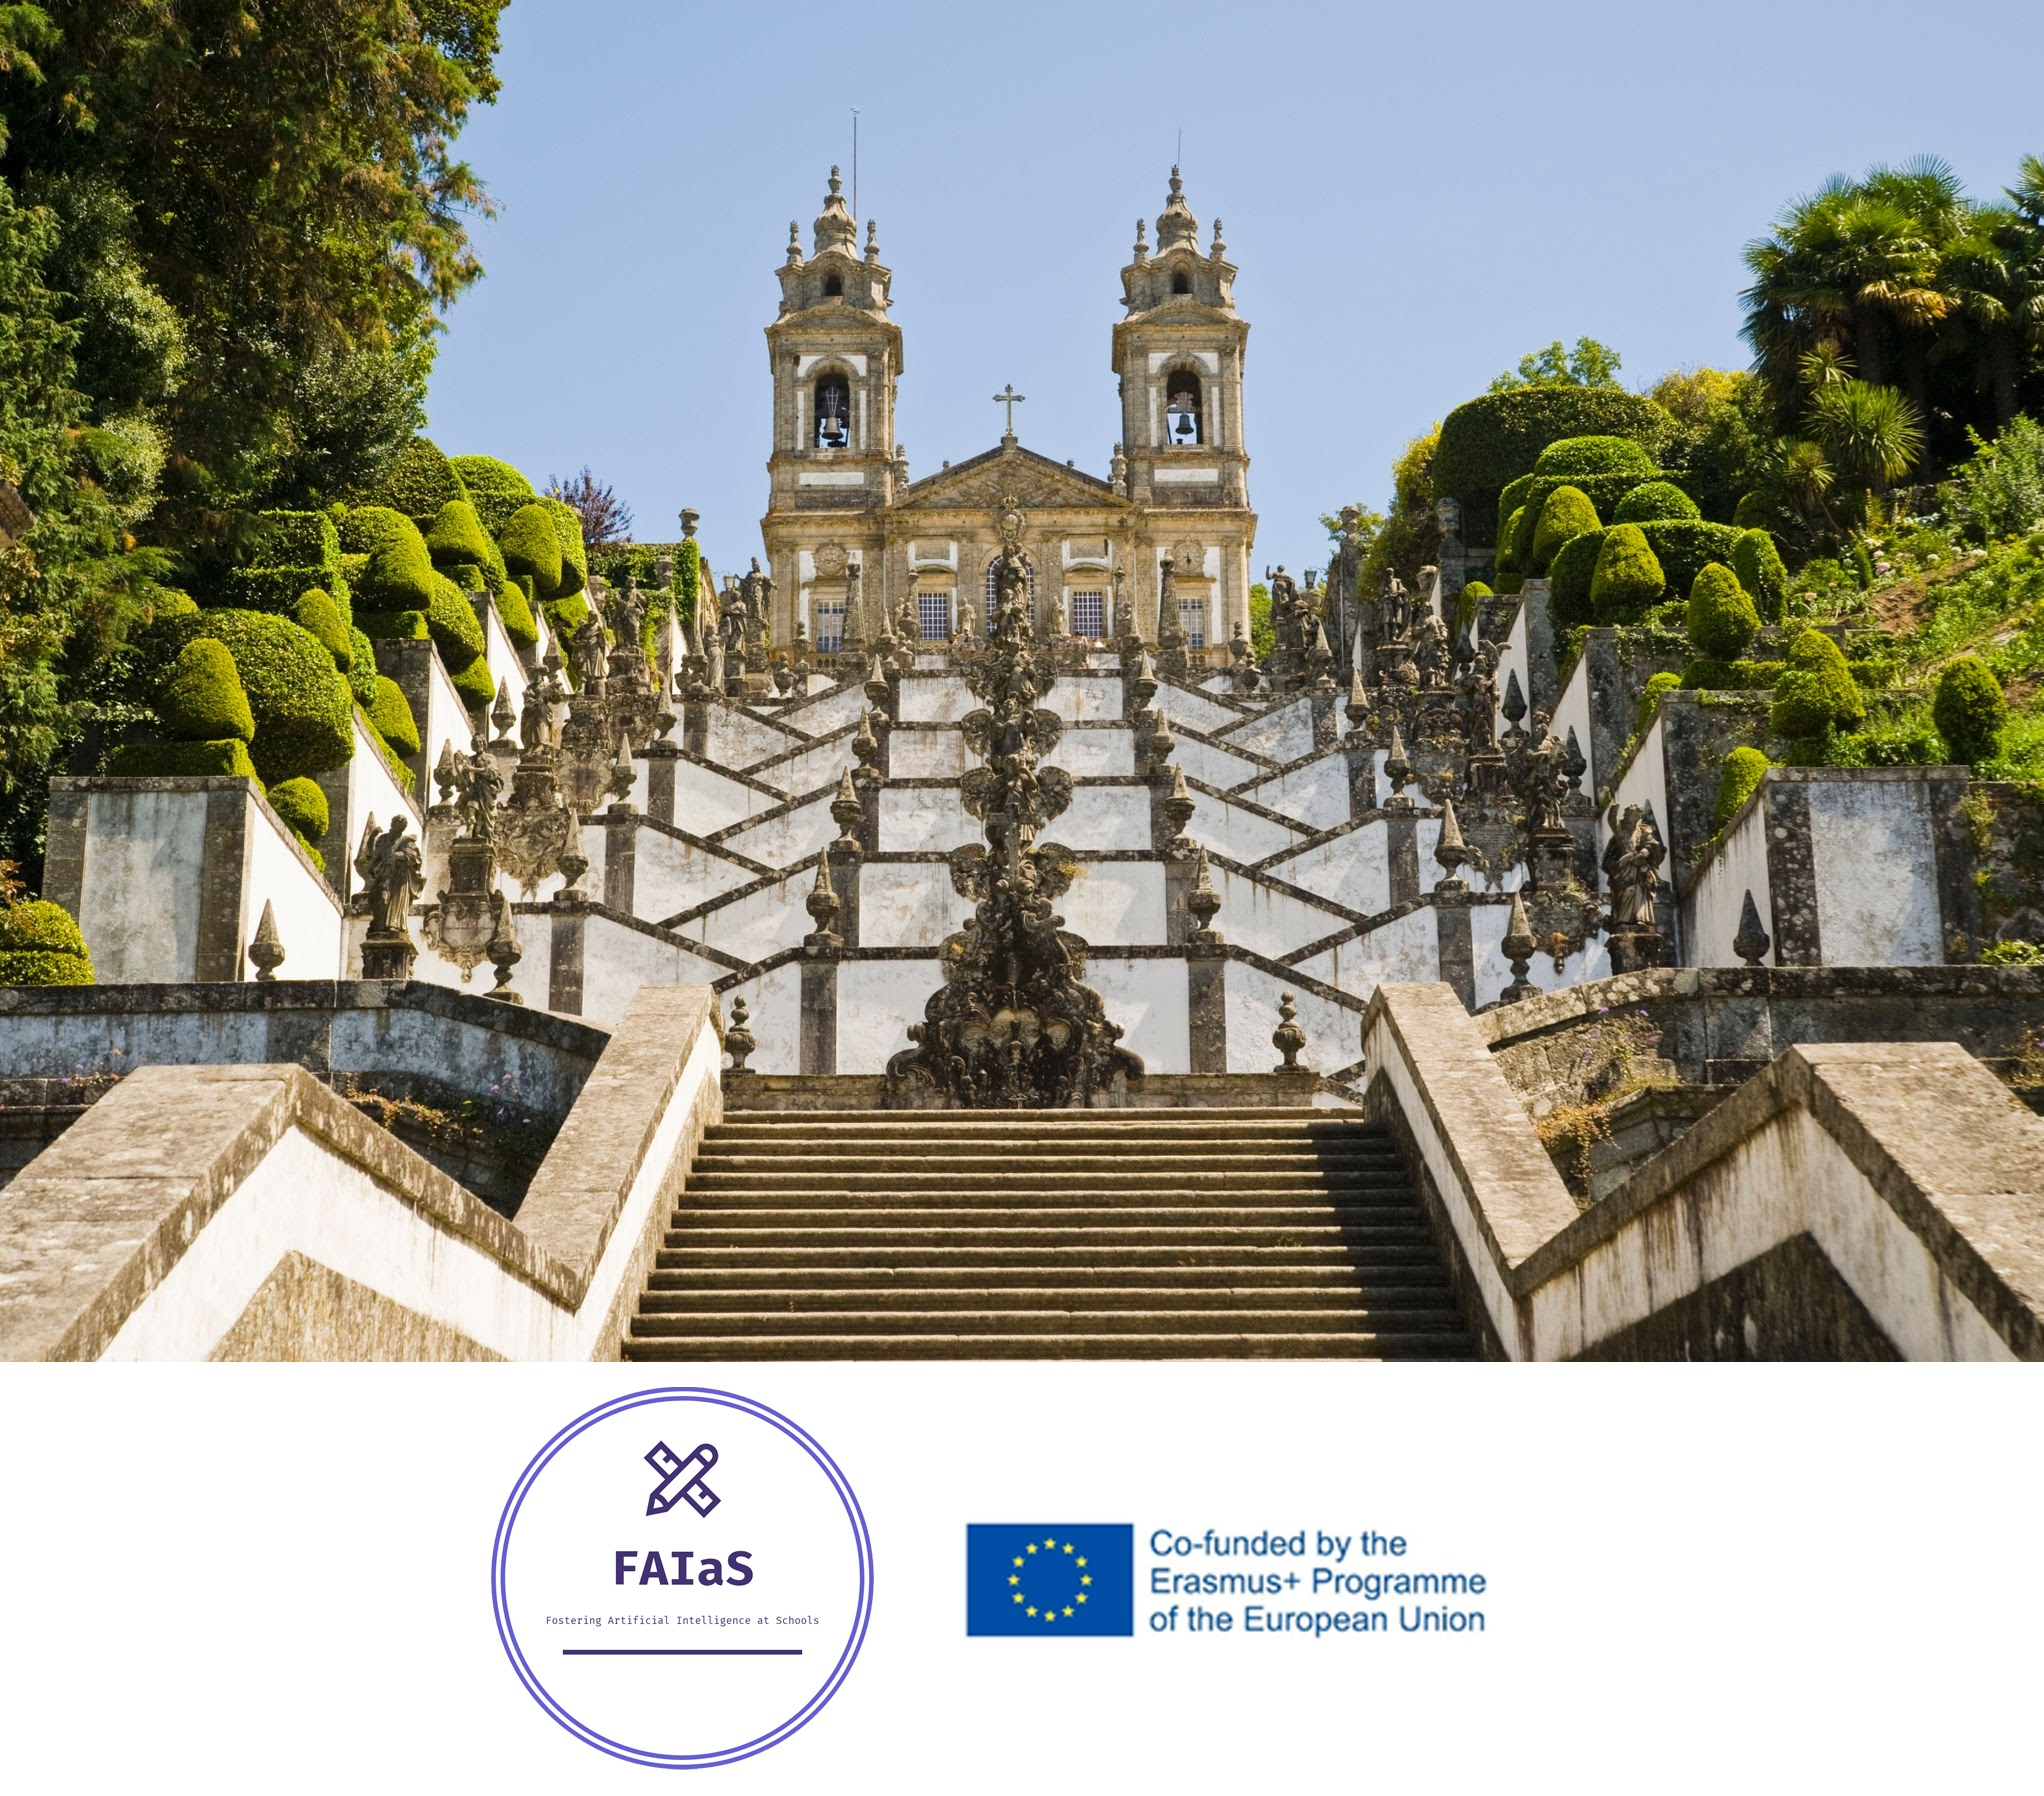
\includegraphics[width=14cm]{logoBraga+faias.jpeg}%
\vspace{1cm}
\begin{Large}
\\
Training to share knowledge and experiences in implementing AI at schools \\
LTTA June 2022 \\
Braga, Portugal, May 31\textsuperscript{st} - June 3\textsuperscript{rd}, 2022 \\
\end{Large}
\vfill
}}}
%%%
% custom titlepage
\makeatletter
\renewcommand{\maketitle}{
\thispagestyle{empty}
\AddToShipoutPicture*{\BackgroundPic}
\ClearShipoutPicture
%
\phantom{a}
\vfill
\phantom{a}\hfill
\begin{tabular}[c]{@{}p{0.7\textwidth}@{}}
      \color{white}\headingfont\LARGE\@title\\[1em]
      \color{white}\headingfont\Large\@author\\[2em]
\end{tabular}
%
\clearpage
}
\makeatother
%%%


%%% fancy boxes
\usepackage{tcolorbox}
\usepackage{wrapfig}
%\def\namesurname{\color{xº}\headingfont\bfseries\uppercase}{\thesubsubsection}{1em}{}

\def\fullboxbegin{
\bigskip
\begin{tcolorbox}[colback=color1,colframe=color1,coltext=white,arc=0mm,boxrule=0pt]
}
\def\fullboxend{\end{tcolorbox}\medskip}
%
\def\leftboxbegin{
\begin{wrapfigure}{l}{0.5\textwidth}
\begin{tcolorbox}[colback=color1,colframe=color1,coltext=white,arc=0mm,boxrule=0pt]
}
\def\leftboxend{
\end{tcolorbox}
\end{wrapfigure}
}
%
\def\rightboxbegin{
\begin{wrapfigure}{r}{0.5\textwidth}
\begin{tcolorbox}[colback=color1,colframe=color1,coltext=white,arc=0mm,boxrule=0pt]
}
\def\rightboxend{
\end{tcolorbox}
\end{wrapfigure}
}
%
\newcounter{frames}
\def\frameboxbegin#1{
\bigskip
\refstepcounter{frames}
\begin{tcolorbox}[colback=white,colframe=color1,arc=0mm,title={\MakeUppercase{#1}}]
}
\def\frameboxend{
\end{tcolorbox}
}
%%%


\usepackage{lipsum}
%\usepackage[spanish]{babel}

\usepackage{booktabs}
\usepackage{array}
\usepackage{tabularx,multirow}

%\setcounter{page}{0}

%%%%%%%%%%%%%%%
% Title Page
\title{}
\author{}
\date{}
%%%%%%%%%%%%%%%

\begin{document}
\maketitle

%\tableofcontents
\clearpage
\clearpage
\section*{Welcome!}
Welcome to the beautiful city of Braga! We are very happy that you all have joined us for this LTTA (learning, teaching and training activities), where we are going to talk and learn about Artificial Intelligence, all within the scope of the FAIaS project. 

This LTTA will be quite informal, but it will serve as a networking point to meet people from very different places (such as Portugal, Spain or Belgium), we will have some good food together and last but not least we will have lots of fun. 

FAIaS fosters the knowledge and skills around Artificial Intelligence and Machine Learning at European schools, funded under an Erasmus+ KA201 innovation in schools project. The project will run until August 2023.

The goals of FAIaS are: 
\begin{enumerate}
    \item To foster the knowledge and skills around Artificial Intelligence and Machine Learning in European schools.
    \item To achieve goal \#1 in a way that is as inclusive as possible, with special attention to gender, economically and socially disadvantaged students, among others. 
    \item To raise awareness of the technical, social and ethical implications of Artificial Intelligence and Machine Learning.
\end{enumerate}

Its expected outcomes are:
\begin{enumerate}
    \item High-quality, open learning materials and experiences for educators and learners on AI and ML.
    \item Easy-to-use web-based (open source) software tools to support learning of AI and ML.
    \item Organization of activities for educators and learners on AI and ML (and make our learning materials, experiences and tools known).
\end{enumerate}


\subsection*{About the LTTA}

During the short-term training activity (4 days) organized in Braga during the next days, the 20 FAIAS educators selected by the partners from the participating countries (9 from Belgium, 6 from Spain and 5 from Portugal) will meet the FAIaS partners and not only will be fully trained on the FAIaS objectives and introduced to the FAIAS outputs, but, most of all, they will be officially designated and invested with their role within the FAIaS project and become a FAIaS Ambassador.

To be FAIaS Ambassador means to be ready, eager and willing to collaborate, contribute, and be committed to the FAIaS project implementation. FAIaS Ambassadors will be a core figure within the project and the role will consist of and will require to:
\begin{itemize}
    \item Contribute in the drafting and revision of the main project outputs (collecting also contributions and suggestions from the local teachers)
    \item Act as a liaison between the FAIaS partners and the FAIaS local teachers communities 
    \item Train and support the local school teachers and colleagues to actively take part to FAIAS activities
    \item Encourage teachers to collaborate, to share ideas and projects, to use the FAIAS repository and tools 
    \item Moderate the FAIaS local community 
    \item Support with the dissemination of the FAIaS results to the school communities
\end{itemize}

During the short-term training activity the FAIaS ambassadors will not only be “theoretically” trained on the FAIAS results. Interactive and collaborative sessions will be organized in order to share experience and proposals between the FAIaS Ambassadors and foster a strong collaboration among them.

\subsection*{Important Places}

Meeting place: 
gnration.
Praça Conde de Agrolongo 

Breakfast:
Doce Carmo.
R. do Carmo

Lunches:
Mostarda e Chocolate.
Praça Conde de Agrolongo

Dinners (Tuesday and Thursday):
Atravessado.
R. de Santo António das Travessas 30

Banquet (Wednesday):
Bem-me-quer.
Campo das Hortas, 6


In the following map you cand find the different sites of interest for the activity.

\begin{figure}[ht]
    \centering
    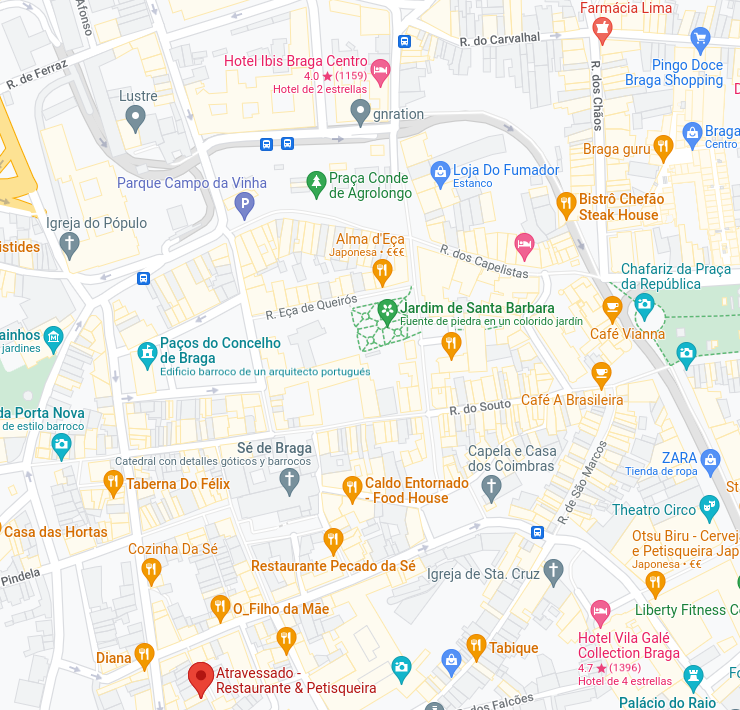
\includegraphics[scale=0.5, keepaspectratio]{braga_map.png}
    \caption{Braga map}
    \label{figure:map}
 \end{figure}

\begin{table}
    \renewcommand{\arraystretch}{1.4}
     \begin{center}
     %\rowcolors{2}{gray!15}{white}
      \begin{tabular}{m{6cm} m{8cm}} % 2 cols 
        \hline
        \rowcolor{gray!35}\centering\arraybackslash\textbf{Day} & \centering\arraybackslash\textbf{Activity} \\
        \hline%\hline
        
        %\rowcolor{white}\multirow[t]{-2}{*}{\textbf{Tuesday, May 31 2022}} & \textbf{16:00 Welcome}(and activity)
        \centering\textbf{Tuesday, May 31 2022} &  \textbf{16:00 Welcome} (and activity) \newline
        \textbf{17:30 Talks by participants} \newline
        - ``Machine Learning in Education'' by Pablo Dúo Terrón \newline
        - ``Overview of AI activities developed by la Scientothèque'' by Yann-Aël Le Borgne \newline
        - ``The use of filters in a deep neural network for image recognition'' by Natacha Gesquière
        \newline
        \textbf{19:00 End} \newline
        \textbf{20:00 Dinner}
        \\ %\hline
        %\cdashline{2-3}
        \rowcolor{gray!15}
        \centering\textbf{Wednesday, June 1 2022} & \textbf{09:30 Breakfast} \newline \textbf{10:00 Intro to AI} \newline \textbf{13:00 Lunch} \newline 
        \textbf{15:00 Talks by participants II} \newline
        - ``AI Generation'' by Maria Inmaculada Caruana\newline
        - ``XR in education'' by Peter De Deyn \newline
        - ``Problem solving with Machine Learning and Scratch'' by Álvaro Molina
        \newline
        \textbf{16:15 LearningML} \newline
        \textbf{17:30 Guided visit through Braga} \newline
        \textbf{19:00 End} \newline
        \textbf{20:00 Banket}
        \\ 
        \centering\textbf{Thursday, June 2 2022} & \textbf{09:30 Breakfast} \newline \textbf{10:00 Example lessons} % Machine Learning in Citizenship lessons by Liliana Carrillo 
        \newline \textbf{13:00 Lunch} \newline
        \textbf{15:00 Preparation:} Create your lesson
        \newline
        \textbf{17:00 Presentations} \newline
        \textbf{17:30 End} \newline
        \textbf{20:00 Dinner} \\
        \rowcolor{gray!15}
        \centering\textbf{Friday, June 3 2022} &
        \textbf{09:30 Breakfast} \newline 
        \textbf{10:00 Presentation time} \newline 
        \textbf{12:00 Reflection and discussion time} \newline 
        \textbf{13:00 Lunch and farewell} \\
        \bottomrule%\hline
    \end{tabular}
      \caption[LTTA program]{LTTA program.}
      \label{tab:program}
     \end{center}
    \end{table}

    \newpage

\section*{Participants}
\noindent
\begin{minipage}{0.3\textwidth}
\centering
\includegraphics[height=5cm]{images/img1.png}
\end{minipage}
\hfill
\begin{minipage}{0.6\textwidth}\raggedright
\color{color1}\uppercase{\textbf{Luis Miguel Iglesias Albarrán}}
\color{color2}\hspace{0.2cm}\includegraphics{flags/es.png}
\hspace{0.2cm}\textit{@luismiglesias}
\\
Secondary School Principal \& Secondary school math teacher and computing and robotics at Instituto de Educación Secundaria 'San Antonio' (Bollullos Par del Condado, Huelva, Andalucía, España)\\
{\footnotesize Married with Teresa. Father of Marta and Juan. Defender of the curricular blog and ICT as basic learning tools, natural extensions of the classroom. Admin of MatemáTICas: 1,1,2,3,5,8,13,... website. Teacher trainer, digital educational content creator, speaker at national educational events and co-author of books sand publications on mathematics, innovation and ICT.}\\
\includegraphics[height=0.35cm]{figs/internet.png}\hspace{0.1cm}{\footnotesize \color{color1}\url{https://luismiglesias.es/}}
\end{minipage}
\newline\newline\newline

\noindent
\begin{minipage}{0.3\textwidth}
\centering
\includegraphics[height=5cm]{images/img2.jpeg}
\end{minipage}
\hfill
\begin{minipage}{0.6\textwidth}\raggedright
\color{color1}\uppercase{\textbf{Ana }}
\color{color2}\hspace{0.2cm}\includegraphics{flags/pt.png}
\\
Elementary school teacher at Caridade\\
{\footnotesize My name is Ana and I am 49 years old. I have been a teacher for 28 years in Guimarães. I am a teacher of EMRC, Arts Education, Dance and I belong to the School Library team. I create educational projects based on children's literature.
I love being a teacher!}\\
\includegraphics[height=0.35cm]{figs/internet.png}\hspace{0.1cm}{\footnotesize \color{color1}\url{https://www.facebook.com/anacaridade.contosterra}}
\end{minipage}
\newline\newline\newline

\noindent
\begin{minipage}{0.3\textwidth}
\centering
\includegraphics[height=5cm]{images/img3.png}
\end{minipage}
\hfill
\begin{minipage}{0.6\textwidth}\raggedright
\color{color1}\uppercase{\textbf{Álvaro Molina Ayuso}}
\color{color2}\hspace{0.2cm}\includegraphics{flags/es.png}
\hspace{0.2cm}\textit{@molinaayuso}
\\
Secondary school teacher at IES Blas Infante\\
{\footnotesize Degree in Physics at the University of Cordoba and teacher of Mathematics in Secondary Education. I currently collaborate with with different educational programmes and initiatives, both nationally and internationally:Scientix ambassador in Spain, Leading Teacher of Europe Code Week, member of the group micro:bit Champions 2022, ambassador of CoSpaces Edu in Spain and member of the Career Adviser Network of STE(A)MIT}\\
\includegraphics[height=0.35cm]{figs/internet.png}\hspace{0.1cm}{\footnotesize \color{color1}\url{https://orcid.org/0000-0001-5948-516X}}
\end{minipage}
\newline\newline\newline

\noindent
\begin{minipage}{0.3\textwidth}
\centering
\includegraphics[height=5cm]{images/img4.jpeg}
\end{minipage}
\hfill
\begin{minipage}{0.6\textwidth}\raggedright
\color{color1}\uppercase{\textbf{Antonio José Romero Barrera}}
\color{color2}\hspace{0.2cm}\includegraphics{flags/es.png}
\hspace{0.2cm}\textit{@ingeniero\_aero}
\\
Researcher at Universidad Rey Juan Carlos\\
{\footnotesize AI researcher at Universidad Rey Juan Carlos. Aerospace Engineering student (Aerospace Vehicles specialization). I have been working five years as aerodynamicist and graphic designer at Ü-Motosport Formula Student team. My hair color changes every month.}\\
\includegraphics[height=0.35cm]{figs/internet.png}\hspace{0.1cm}{\footnotesize \color{color1}\url{https://gestion2.urjc.es/pdi/ver/antonio.romero}}
\end{minipage}
\newline\newline\newline

\noindent
\begin{minipage}{0.3\textwidth}
\centering
\includegraphics[width=5cm]{images/img5.jpeg}
\end{minipage}
\hfill
\begin{minipage}{0.6\textwidth}\raggedright
\color{color1}\uppercase{\textbf{Marjon Blondeel}}
\color{color2}\hspace{0.2cm}\includegraphics{flags/be.png}
\\
Software/AI developer at VUB\\
{\footnotesize Researcher in AI until 2015. Now focused on developing AI applications and giving trainings on AI. During 1 year I also worked as a teacher in secondary school and I have many years of experience as a teaching assistant and lecturer in higher education. I've taught basic courses for informatics students, but also programming courses for other students such as Bio-Engineering students. }\\
\end{minipage}
\newline\newline\newline

\noindent
\begin{minipage}{0.3\textwidth}
\centering
\includegraphics[height=5cm]{images/img6.jpeg}
\end{minipage}
\hfill
\begin{minipage}{0.6\textwidth}\raggedright
\color{color1}\uppercase{\textbf{Sara Borges}}
\color{color2}\hspace{0.2cm}\includegraphics{flags/pt.png}
\\
Program Assistant at Braga Media Arts / Teatro Circo de Braga\\
{\footnotesize I'm a program assistant at Circuito - Braga Media Arts Educational Service. I'm also part of the team hosting the event, so please feel free to contact if needed! 
}\\
\end{minipage}
\newline\newline\newline

\noindent
\begin{minipage}{0.3\textwidth}
\centering
\includegraphics[height=5cm]{images/img7.jpeg}
\end{minipage}
\hfill
\begin{minipage}{0.6\textwidth}\raggedright
\color{color1}\uppercase{\textbf{Yann-Aël Le Borgne}}
\color{color2}\hspace{0.2cm}\includegraphics{flags/fr.png}
\hspace{0.2cm}\textit{@ya\_lb}
\\
Developer of educational resources at La Scientothèque ASBL\\
{\footnotesize My background is in academia, in fields related to cognitive sciences and artificial intelligence (AI). I worked as a researcher for 15 years at the University of Brussels, in the Machine Learning Group of the Department of Computer Science. I recently joined La Scientothèque, where I currently develop educational resources on AI for young audiences.}\\
\includegraphics[height=0.35cm]{figs/internet.png}\hspace{0.1cm}{\footnotesize \color{color1}\url{https://yannael.github.io/}}
\end{minipage}
\newline\newline\newline

\noindent
\begin{minipage}{0.3\textwidth}
\centering
\includegraphics[height=5cm]{images/img8.jpeg}
\end{minipage}
\hfill
\begin{minipage}{0.6\textwidth}\raggedright
\color{color1}\uppercase{\textbf{Liliana Carrillo}}
\color{color2}\hspace{0.2cm}\includegraphics{flags/es.png}
\hspace{0.2cm}\textit{@lilicarrillof}
\\
Founding Director at CollectiveUP\\
{\footnotesize I am a very curious person, eager to learn, and that has brought me to innovate in many ways.  I am a computer science engineer with a background in AI, business and education, and a passion for social work, and social impact.  I love art, museums, chatting with people, and a good meal.}\\
\includegraphics[height=0.35cm]{figs/internet.png}\hspace{0.1cm}{\footnotesize \color{color1}\url{https://be.linkedin.com/in/carrilloliliana}}
\end{minipage}
\newline\newline\newline

\noindent
\begin{minipage}{0.3\textwidth}
\centering
\includegraphics[height=5cm]{images/img0.jpg}
\end{minipage}
\hfill
\begin{minipage}{0.6\textwidth}\raggedright
\color{color1}\uppercase{\textbf{Macu Caruana}}
\color{color2}\hspace{0.2cm}\includegraphics{flags/es.png}
\hspace{0.2cm}\textit{@macucaruana}
\\
Primary Teacher at Teacher\\
{\footnotesize Keen on Technology and education. I love sports, fan of Rafa Nadal. I also like photography and living as close as possible to the sea.}\\
\end{minipage}
\newline\newline\newline

\noindent
\begin{minipage}{0.3\textwidth}
\centering
\includegraphics[height=5cm]{images/img10.jpeg}
\end{minipage}
\hfill
\begin{minipage}{0.6\textwidth}\raggedright
\color{color1}\uppercase{\textbf{Hannes Cools}}
\color{color2}\hspace{0.2cm}\includegraphics{flags/be.png}
\hspace{0.2cm}\textit{@CoolsHannes}
\\
PhD-researcher and lecturer at KU Leuven\\
{\footnotesize 
Hannes Cools is a PhD candidate at the Institute for Media Studies, KU Leuven, Belgium. His research interests include AI, computational journalism and news automation. He is also an affiliated researcher at Georgetown University in Washington DC. }\\
\includegraphics[height=0.35cm]{figs/internet.png}\hspace{0.1cm}{\footnotesize \color{color1}\url{https://www.linkedin.com/in/hannes-cools-18a16323/}}
\end{minipage}
\newline\newline\newline

\noindent
\begin{minipage}{0.3\textwidth}
\centering
\includegraphics[height=5cm]{images/img11.png}
\end{minipage}
\hfill
\begin{minipage}{0.6\textwidth}\raggedright
\color{color1}\uppercase{\textbf{Meritxell Díaz Coque}}
\color{color2}\hspace{0.2cm}\includegraphics{flags/es.png}
\\
Researcher at Universidad Rey Juan Carlos\\
{\footnotesize I am a Electrical Engineer in Telecommunications and in Aerospace Engineer, currently working as a researcher in the FAIaS project. In this project, we are trying to teach Artificial Intelligence in high schools. I'm passionate about programming and artificial intelligence.}\\
\end{minipage}
\newline\newline\newline

\noindent
\begin{minipage}{0.3\textwidth}
\centering
\includegraphics[height=5cm]{images/img0.jpg}
\end{minipage}
\hfill
\begin{minipage}{0.6\textwidth}\raggedright
\color{color1}\uppercase{\textbf{Patricia Corieri}}
\color{color2}\hspace{0.2cm}\includegraphics{flags/be.png}
\hspace{0.2cm}\textit{@patriciacorieri}
\\
DIRECTOR at La Scientothèque ASBL\\
{\footnotesize After working 30 years as a research engineer, and studying pedagogy I decided  to finish my carreer in developing after schools activities for non priviledge area of Brussels and to help in the development of innivative teaching ressources for schools based on a large pratical experince}\\
\includegraphics[height=0.35cm]{figs/internet.png}\hspace{0.1cm}{\footnotesize \color{color1}\url{www.lascientheque.be}}
\end{minipage}
\newline\newline\newline

\noindent
\begin{minipage}{0.3\textwidth}
\centering
\includegraphics[height=5cm]{images/img13.jpeg}
\end{minipage}
\hfill
\begin{minipage}{0.6\textwidth}\raggedright
\color{color1}\uppercase{\textbf{Romeu Gonçalo Ramos Ferreira da Costa}}
\color{color2}\hspace{0.2cm}\includegraphics{flags/pt.png}
\\
All school levels Saxophone Teacher at Conservatório de Música Calouste Gulbenkian de Braga\\
{\footnotesize I consider myself a musician who, at the same time, teaches. The stage experience is of great value to me and I try to carry it into the classroom. As a teacher, I have had the opportunity to work in all music education systems in Portugal, covering all age groups. The subject I teach (Instrument - Saxophone) is characterized by being practical and individual - 1 teacher and 1 student in each class.}\\
\end{minipage}
\newline\newline\newline

\noindent
\begin{minipage}{0.3\textwidth}
\centering
\includegraphics[height=5cm]{images/img14.jpeg}
\end{minipage}
\hfill
\begin{minipage}{0.6\textwidth}\raggedright
\color{color1}\uppercase{\textbf{Peter De Deyn}}
\color{color2}\hspace{0.2cm}\includegraphics{flags/be.png}
\\
IT advisor at Brothers of Charity\\
{\footnotesize I'm very interested in  technology especially in education but also in a broader scope. My work and drive is to motivate users to integrate and make use of new technologies into their teaching and daily life.}\\
\end{minipage}
\newline\newline\newline

\noindent
\begin{minipage}{0.3\textwidth}
\centering
\includegraphics[height=5cm]{images/img15.jpeg}
\end{minipage}
\hfill
\begin{minipage}{0.6\textwidth}\raggedright
\color{color1}\uppercase{\textbf{Natacha Gesquière}}
\color{color2}\hspace{0.2cm}\includegraphics{flags/be.png}
\hspace{0.2cm}\textit{@NachaGesquiere}
\\
STEM coach at UGent - AIRO - IDLab \\
{\footnotesize Natacha Gesquière is a master in mathematics and media coach. She was a math teacher for many years in secondary school, but now she is a STEM coach at Ghent University and Dwengo. She developpes lesson materials about STEM, computational thinking, artificial intelligence, and programming. }\\
\includegraphics[height=0.35cm]{figs/internet.png}\hspace{0.1cm}{\footnotesize \color{color1}\url{https://www.aiopschool.be/}}
\end{minipage}
\newline\newline\newline

\noindent
\begin{minipage}{0.3\textwidth}
\centering
\includegraphics[height=5cm]{images/img0.jpg}
\end{minipage}
\hfill
\begin{minipage}{0.6\textwidth}\raggedright
\color{color1}\uppercase{\textbf{Chrysanthi Katrini}}
\color{color2}\hspace{0.2cm}\includegraphics{flags/gr.png}
\\
Senior AI Coach \& AI Coordinator at BeCode\\
{\footnotesize I am Chrysanthi, 31 years old woman with a child dream to make free education for everyone a must. In combination with my background in Computer Science and Artificial Intelligence I managed to work in several envs, from a University to where I am now, an Non Profit ogranization with a scope of coaching learners programming languages and prepare them for the market. I like walking , board games and reading books. }\\
\end{minipage}
\newline\newline\newline

\noindent
\begin{minipage}{0.3\textwidth}
\centering
\includegraphics[height=5cm]{images/img0.jpg}
\end{minipage}
\hfill
\begin{minipage}{0.6\textwidth}\raggedright
\color{color1}\uppercase{\textbf{Johan Loeckx}}
\color{color2}\hspace{0.2cm}\includegraphics{flags/be.png}
\hspace{0.2cm}\textit{@aibrussels}
\\
Researcher at Artificial Intelligence Lab Brussels (VUB)\\
{\footnotesize I have three passions: music, education \& AI.  have founded a Freinet school in Brussels, I have done research on using AI to educate people on music, and am currently mainly involved with lifelong learning of AI.}\\
\end{minipage}
\newline\newline\newline

\noindent
\begin{minipage}{0.3\textwidth}
\centering
\includegraphics[height=5cm]{images/img0.jpg}
\end{minipage}
\hfill
\begin{minipage}{0.6\textwidth}\raggedright
\color{color1}\uppercase{\textbf{Joana Miranda}}
\color{color2}\hspace{0.2cm}\includegraphics{flags/pt.png}
\\
General executive Coordinator of BMA at Teatro Circo de Braga/Braga Media Arts\\
{\footnotesize Joana Miranda is a new media strategist and training expert, creative media producer and educator currently working as Executive general Coordinator at Braga Media Arts [Unesco Creative City] at Teatro Circo de Braga, EM, SA.}\\
\includegraphics[height=0.35cm]{figs/internet.png}\hspace{0.1cm}{\footnotesize \color{color1}\url{https://we.tl/t-fpnoMOYn79}}
\end{minipage}
\newline\newline\newline

\noindent
\begin{minipage}{0.3\textwidth}
\centering
\includegraphics[height=5cm]{images/img19.jpeg}
\end{minipage}
\hfill
\begin{minipage}{0.6\textwidth}\raggedright
\color{color1}\uppercase{\textbf{Ainhoa Erize Mota}}
\color{color2}\hspace{0.2cm}\includegraphics{flags/es.png}
\hspace{0.2cm}\textit{@ainhoaberrilasa}
\\
ICT assessor at ICT assessor. Innovation centre for schools. Basque Country Spain\\
{\footnotesize I'm an English teacher at Primary school, but right now working as an ICT assessor in an Innovation Centre for schools and teachers. I love technology and I'm councious of all the benefits of it at education. Appart from that, trying to understand how our society is developing, I'd like helping the rest, schools and teachers, understanding the benefits of our new world. }\\
\end{minipage}
\newline\newline\newline

\noindent
\begin{minipage}{0.3\textwidth}
\centering
\includegraphics[height=5cm]{images/img20.png}
\end{minipage}
\hfill
\begin{minipage}{0.6\textwidth}\raggedright
\color{color1}\uppercase{\textbf{CRISTIAN RUIZ}}
\color{color2}\hspace{0.2cm}\includegraphics{flags/es.png}
\hspace{0.2cm}\textit{@sigueacristian}
\\
IT Head \& Computer Science Teacher at COLEGIO JUAN DE LANUZA, ZARAGOZA (SPAIN)\\
{\footnotesize I enjoy my work, I do what I like the most and what I know how to do best: teaching. I have worked in all educational stages and in all areas.

I am passionate about everything that has to do with the use of new technologies in a pedagogical way in the classroom. I consider it essential that students learn programming and robotics from a very young age, in order to stimulate their thinking skills.}\\
\includegraphics[height=0.35cm]{figs/internet.png}\hspace{0.1cm}{\footnotesize \color{color1}\url{www.openlanuza.com}}
\end{minipage}
\newline\newline\newline

\noindent
\begin{minipage}{0.3\textwidth}
\centering
\includegraphics[height=5cm]{images/img21.jpeg}
\end{minipage}
\hfill
\begin{minipage}{0.6\textwidth}\raggedright
\color{color1}\uppercase{\textbf{Gregorio Robles}}
\color{color2}\hspace{0.2cm}\includegraphics{flags/es.png}
\hspace{0.2cm}\textit{@gregoriorobles}
\\
Full Professor at Universidad Rey Juan Carlos\\
{\footnotesize I am a Full Professor at the Universidad Rey Juan Carlos, a public university in the South of Madrid.}\\
\includegraphics[height=0.35cm]{figs/internet.png}\hspace{0.1cm}{\footnotesize \color{color1}\url{https://gsyc.urjc.es/~grex/}}
\end{minipage}
\newline\newline\newline

\noindent
\begin{minipage}{0.3\textwidth}
\centering
\includegraphics[width=5cm]{images/img22.png}
\end{minipage}
\hfill
\begin{minipage}{0.6\textwidth}\raggedright
\color{color1}\uppercase{\textbf{Elaine Vianna Saraiva}}
\color{color2}\hspace{0.2cm}\includegraphics{flags/br.png}
\hspace{0.2cm}\textit{@elaineviann}
\\
Teacher at Duodifusão\\
{\footnotesize 
Researcher, teacher and actress. I have a  post doctorate in Communication Sciences. I am an expert in trademarks and have been an examiner at the Brazilian Institute of Industrial Property  for 20 years. Currently, I work as a teacher and trainer in professional training courses in the areas of art, education and communication.
In addition, I promote poetic expression activities, such as soirees and workshops.}\\
\includegraphics[height=0.35cm]{figs/internet.png}\hspace{0.1cm}{\footnotesize \color{color1}\url{https://www.instagram.com/movimentopoesie\_se/}}
\end{minipage}
\newline\newline\newline

\noindent
\begin{minipage}{0.3\textwidth}
\centering
\includegraphics[height=5cm]{images/img0.jpg}
\end{minipage}
\hfill
\begin{minipage}{0.6\textwidth}\raggedright
\color{color1}\uppercase{\textbf{Pedro Miguel Amaro Correia Sequeira}}
\color{color2}\hspace{0.2cm}\includegraphics{flags/pt.png}
\\
High school teacher at Public school\\
{\footnotesize  teacher who likes to learn}\\
\end{minipage}
\newline\newline\newline

\noindent
\begin{minipage}{0.3\textwidth}
\centering
\includegraphics[height=5cm]{images/img24.jpeg}
\end{minipage}
\hfill
\begin{minipage}{0.6\textwidth}\raggedright
\color{color1}\uppercase{\textbf{Madhumalti Sharma}}
\color{color2}\hspace{0.2cm}\includegraphics{flags/lu.png}
\hspace{0.2cm}\textit{@workshop4me}
\\
Founder and President, Educator at Workshop4Me a.s.b.l.\\
{\footnotesize More than 25 years in tech, founded Workshop4Me a.s.b.l., to create the problem solvers of the future using technology. EU Code Week Ambassador, EU Robotics National Coordinator, Executive Board of European Association of STEAM Educators, Country Chair for Robotics and Automation at G100:Mission Million. Instrumental in bringing coding into the primary school curriculum in Luxembourg. Author of ‘Let’s Code Python’}\\
\includegraphics[height=0.35cm]{figs/internet.png}\hspace{0.1cm}{\footnotesize \color{color1}\url{https://workshop4me.org/our-team-1}}
\end{minipage}
\newline\newline\newline

\noindent
\begin{minipage}{0.3\textwidth}
\centering
\includegraphics[width=5cm]{images/img25.png}
\end{minipage}
\hfill
\begin{minipage}{0.6\textwidth}\raggedright
\color{color1}\uppercase{\textbf{Pablo Duo Terron}}
\color{color2}\hspace{0.2cm}\includegraphics{flags/es.png}
\hspace{0.2cm}\textit{@esparaTIC}
\\
Director and teacher  in Primary School at ministry of education and vocational training\\
{\footnotesize Doctoral student in education 
Master TIC and Educational Inspection 
Degree in primary school and physical education  
2nd best teacher of Primary School in Spain 2021
Coordinator and tutor of the Future Classroom courses of the (national institute of technology teacher training in Spain) INTEF
Tutor of the Computational Thinking and Artificial Intelligence school of the INTEF
STEM Diagnostic Test Coordinator INEE}\\
\includegraphics[height=0.35cm]{figs/internet.png}\hspace{0.1cm}{\footnotesize \color{color1}\url{https://www.educaciontic.es}}
\end{minipage}
\newline\newline\newline

\noindent
\begin{minipage}{0.3\textwidth}
\centering
\includegraphics[width=5cm]{images/img26.jpeg}
\end{minipage}
\hfill
\begin{minipage}{0.6\textwidth}\raggedright
\color{color1}\uppercase{\textbf{Robbe Wulgaert}}
\color{color2}\hspace{0.2cm}\includegraphics{flags/be.png}
\hspace{0.2cm}\textit{@RWulgaert}
\\
Teacher at Sint-Lievenscollege Gent\\
{\footnotesize I am a programming, Artificial Intelligence and Design Thinking teacher in Ghent. You can usally find me in my classroom as a full-time teacher at Sint-Lievenscollege or as an external assistant at the University of Ghent. In my spare time I am endlessly fascinated by education, photography and (anamorphic) videography. A hobby that got out of hand, or rather, I turned my interests into my profession, who knows?}\\
\includegraphics[height=0.35cm]{figs/internet.png}\hspace{0.1cm}{\footnotesize \color{color1}\url{https://www.robbewulgaert.be/about}}
\end{minipage}
\newline\newline\newline



\newpage
\begin{center}
\Huge \textbf{Notes}
\end{center}

\end{document}
